% -*- mode: latex; mode: auto-fill; coding: utf-8; -*-

\section{Linear Transformations}
\label{sec:linear_transformation}
A linear transformation, or linear mapping, is a function $f$ that maps
one vector space into another with the property that\citebook{page~175}{book:leon}:

\begin{equation}
f(\alpha x + \beta y) = \alpha f(x) + \beta f(y)
\end{equation}

where $\alpha$ and $\beta$ are scalars.
An \defit{affine} transformation from a Euclidean space into another is
a mapping which preserves collinearity of points and ratios of
distances between points on a straight line. In other words, points which lie
on a straight line before the transformation continue to do so after the transformation is
applied. Consider point $a$, $b$ and $c$, the ratio $\frac{ \vert
  b-a\vert}{\vert c-b \vert}$ is preserved when using affine transformations.
An affine transformation can be a translation, a rotation, a scaling,
a shear or a combination hereof using matrix
multiplication\citebook{page~2}{book:3d-games}.
%
A common form of a linear equation in two variables, $x$ and $y$ is 

\begin{equation}
\label{eq:linear-equation}
y = A x + b
\end{equation}

where $A$ is a matrix representing rotation, scaling or shearing and
$b$ represents translation. 
The set of solutions to this equation forms a straight line hence the
name linear. Using \defit{homogeneous} coordinates means representing an
$n$-dimensional vector by $(n+1)$ components. This way we can
include translation in the set of affine transformations and hereby get rid of
$b$ in equation \eqref{eq:linear-equation}. 
The following examples shows commonly used affine transformations. \\

\subsection*{Translation}
\label{sec:basic_math_translation}
Here is an example of an affine three-dimensional translation:
\begin{equation}
\label{eq:translation_matrix}
T = 
\begin{bmatrix} 
1 & 0 & 0 & t_x \\ 
0 & 1 & 0 & t_y \\ 
0 & 0 & 1 & t_z \\
0 & 0 & 0 & 1 
\end{bmatrix} 
\end{equation} 

$t_x$, $t_y$ and $t_z$ are the axial translations in the $x$, $y$, and $z$
axis respectively. Only the rightmost column concerns the
translation as opposed to scaling, rotation and shearing where only
the upper-left $3\times3$ sub-matrix defines the transformation.
Any affine transformation matrix can be applied to a vector $4 \times
1$ vector $v$ by using matrix multiplication $v^\prime = T \ v$:

\begin{equation}
%\label{eq:translation_matrix}
\begin{bmatrix} 
x' \\ y' \\ z' \\ 1 
\end{bmatrix} 
= 
\begin{bmatrix} 
1 & 0 & 0 & t_x \\ 
0 & 1 & 0 & t_y \\ 
0 & 0 & 1 & t_z \\
0 & 0 & 0 & 1 
\end{bmatrix} 
\begin{bmatrix} 
x \\ y \\ z \\ 1 
\end{bmatrix}
\end{equation} 

Notice that the fourth vector component has the value one since it is
in homogeneous form. This way translation can be applied using
matrix multiplication instead of the standard vector addition as shown
in equation \eqref{eq:linear-equation}. \\ 

\subsection*{Scaling}
\label{sec:basic_math_scaling}
This is an affine scaling matrix:
%Here is an example of an affine scaling:
\begin{equation}
\label{eq:scaling_matrix}
S = 
\begin{bmatrix} 
S_x & 0 & 0 & 0 \\ 
0 & S_y & 0 & 0 \\ 
0 & 0 & S_z & 0 \\
0 & 0 & 0 & 1 
\end{bmatrix} 
\end{equation} 

$S_x$, $S_y$, and $S_z$ are the scaling factors in the $x$, $y$, and $z$
axis respectively. \\

\subsection*{Shearing}
\label{sec:basic_math_shearing}
Generally shearing can be performed
in an arbitrary plane. There are six basic shearing matrices
\citebook{page~31}{book:realtime}. One for each 
off-diagonal component in the upper-left $3\times3$ matrix as
illustrated here:
 
\begin{equation}
\label{eq:shearing_matrix}
H = 
\begin{bmatrix} 
1 & S_{xy} & S_{xz} & 0 \\ 
S_{yx} & 1 & S_{yz} & 0 \\ 
S_{zx} & S_{zy} & 1 & 0\\
0 & 0 & 0 & 1 
\end{bmatrix} 
\end{equation} 

For simplicity the following example only illustrates
shearing acting in planes orthogonal to axis of the coordinate
frame. The following is an example of a shearing matrix in the
$xy$-plane: 

\begin{equation}
\label{eq:shearing_matrix_xy_plane}
H_{xy} = 
\begin{bmatrix} 
1 & t & 0 & 0 \\ 
0 & 1 & 0 & 0 \\ 
0 & 0 & 1 & 0\\
0 & 0 & 0 & 1 
\end{bmatrix} 
\end{equation} 

The result of applying the $H_{xy}$ shearing matrix to a unit square is
illustrated in figure \vref{fig:mathematics_unit_square_shearing}.


%% Figure showing shearing of unit square.
\begin{figure}
  \centering
  \subfloat[Before]{
    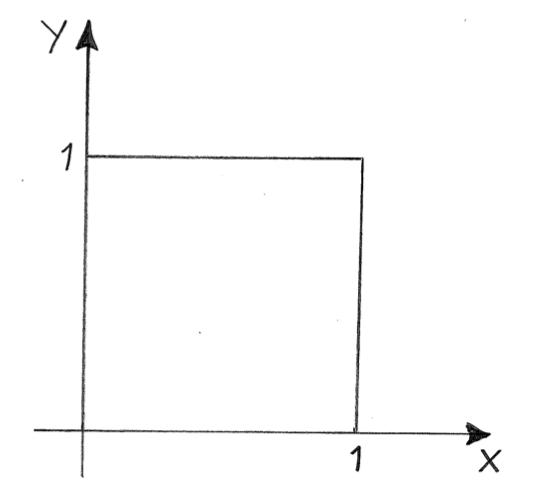
\includegraphics[width=6cm]{./images/mathematics_shearing_unit_square_before.png}
  }
  \subfloat[After]{
    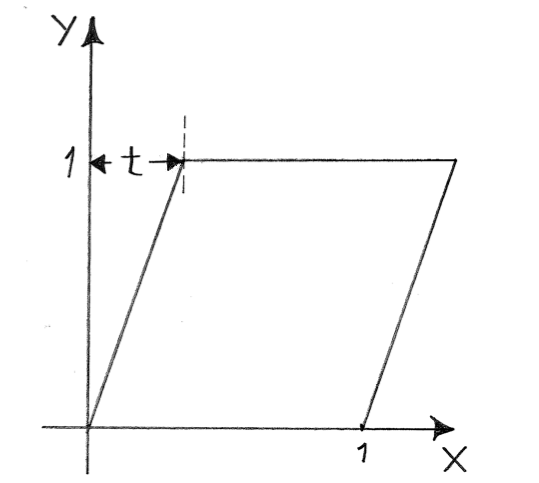
\includegraphics[width=6cm]{./images/mathematics_shearing_unit_square_after.png}
  }
\caption{Shearing in the xy-plane applied to a unit square.}
\label{fig:mathematics_unit_square_shearing}
\end{figure}

\subsection*{Rotation}
\label{sec:basic_math_rotation}
Generally rotation can be applied around an arbitrary axis but for
simplicity the examples here are limited to rotations around the $x$, $y$, and $z$ axis.
The following three examples illustrate counter-clockwise rotation $\theta$ degrees
around the $x$, $y$, and $z$ axis respectively:
\begin{equation}
\label{eq:rotation_matrix_x}
R_x = 
\begin{bmatrix} 
1 & 0 & 0 & 0 \\ 
0 & cos \theta & - sin \theta & 0 \\ 
0 & sin \theta & cos \theta & 0\\
0 & 0 & 0 & 1 
\end{bmatrix} 
\end{equation} 
\begin{equation}
\label{eq:rotation_matrix_y}
R_y = 
\begin{bmatrix} 
cos \theta & 0 & sin \theta & 0 \\ 
0 &  1 & 0 & 0 \\ 
- sin \theta & 0 & cos \theta & 0\\
0 & 0 & 0 & 1 
\end{bmatrix} 
\end{equation} 
\begin{equation}
\label{eq:rotation_matrix_z}
R_z = 
\begin{bmatrix} 
cos \theta & - sin \theta & 0 & 0 \\ 
sin \theta & cos \theta & 0 & 0 \\ 
0 & 0 & 1 & 0\\
0 & 0 & 0 & 1 
\end{bmatrix} 
\end{equation} 

Constructing an affine rotation matrix requires certain matrix
properties. To ensure preservation of collinearity and ratio of
distances between points along lines the rotation matrix must be an
\defit{orthogonal} matrix. An
orthogonal rotation matrix is by definition a square matrix with rows
(or columns) that
form an \defit{orthonormal basis} \citebook{page~258}{book:leon}. An orthonormal
basis is a set of mutually perpendicular vectors all of magnitude
one \citebook{page~255}{book:leon} as illustrated in figure
\vref{fig:orthonormal_basis}.  

\begin{figure}
  \centering
  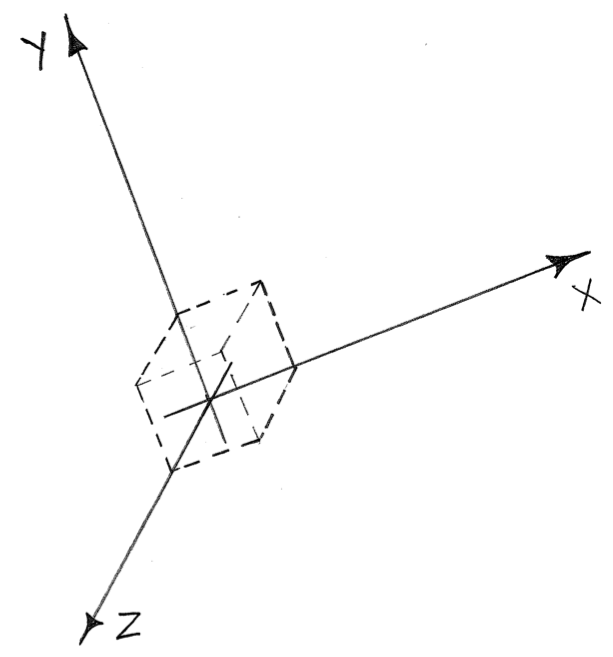
\includegraphics[width=6cm]{./images/mathematics_orthogonal_matrix.png}
\caption{An orthonormal basis.}
\label{fig:orthonormal_basis}
\end{figure}
  
The determinant of any orthogonal matrix is either $+1$ or $-1$. If the
determinant equals $-1$ it forms a reflection matrix rather than a
rotation matrix.
If the determinant of the orthogonal matrix equals $1$ it forms a
rotation matrix and these are the ones we are interested in. 
%
A rotation matrix has the following useful properties:

\begin{itemize}
\item Columns (or rows) are orthogonal unit vectors.
\item The transpose equals the inverse:
\begin{equation}
\label{eq:inverse_equals_transposed}
A A^T = A^T A = A^{-1} A = I
\end{equation}
\item The determinant equals $+1$.
\item Closed under multiplication and the inverse operation. 
\end{itemize}

The fact that the inverse
of a rotation matrix is the same as the transpose is very
useful. The transpose of a matrix can be found just by swapping rows
with columns, whereas finding the inverse usually means solving a system of
linear equations using Gaussian elimination or another solving
technique, so generally transposing a matrix is computationally much
faster. 


\section{Tensors}
\label{sec:tensors}
Tensors are a powerful abstraction proven
very useful especially in physics and engineering. Because of its
abstractness it is not an easy entity to describe. A tensor is a way
of describing linear transformations according to certain rules.
A tensor is in fact just a linear function, but in applied
mathematics it sometimes seems like a ``magic'' entity. \\  


% TENSOR EXAMPLE 
% sailor http://en.wikibooks.org/wiki/General_relativity:What_is_a_tensor%3F
%The use of tensors are probably best explained though examples.

The use of tensors are probably best motivated through an
example. Consider the life of a pirate sailing on the ocean only
powered by the wind.
Dependent on the weather conditions the wind
will have a certain speed and come from a certain direction. Wind could easily
be represented as a vector $v$ where the magnitude of the vector
represents the wind speed. When the wind hits the sail it produces a
force that will make the ship move. If the ship was always sailing in the
same direction as the wind we could just represent the relation between
wind and force with a simple scalar. The resulting
force vector could simply be obtained by multiplying the wind vector with the
scalar. You don't have to be a sailor to see that if the ship
could only move in the direction of the wind only random sailing would
be possible. Sailing is more complicated in real life. We need to
represent the relation between wind and resulting force in a different
way. We shall assume that this relation is linear, so doubling the
wind speed will double the force. We could represent this linear relation
between the wind and the force on matrix form:

\begin{equation}
T = 
\begin{bmatrix} 
\tau_{11} & \tau_{12} \\
\tau_{21} & \tau_{22} \\
\end{bmatrix} 
\end{equation}

Here $T$ is an example of a tensor capable of relating two different quantities,
one is the wind speed and direction the other is the force direction
and magnitude. The resulting force could be expressed as:

\begin{equation}
f = T \cdot w
\end{equation}

where $T$ is the tensor, $w$ and $f$ is the wind and
force vector, respectively.

\begin{figure}
  \centering
  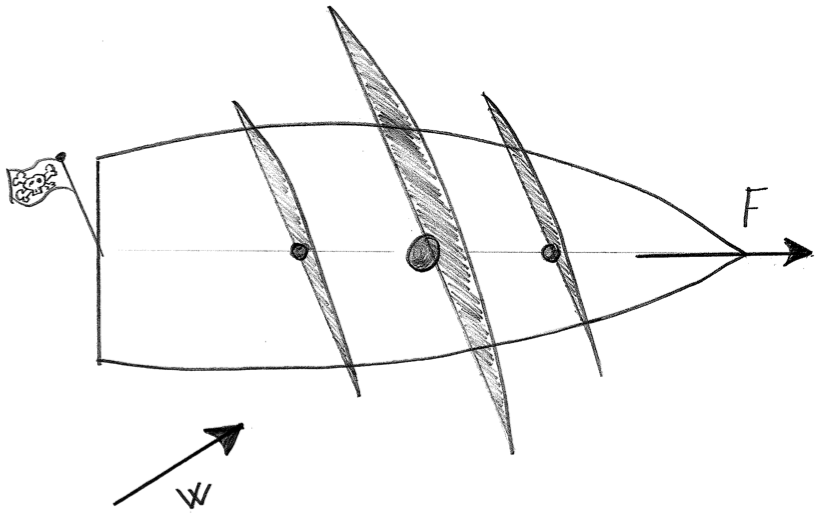
\includegraphics[width=10cm]{./images/mathematics_tensor_pirate_ship.png}
\caption{Wind from behind hits the sail and produces force.}
\label{fig:tensor_pirate_ship}
\end{figure}

As illustrated on figure \vref{fig:tensor_pirate_ship} the pirate ship with its sail set, is
going in a direction say $45^\circ$ to the right of the wind
direction. We represent the wind direction and speed as $w =
[1,1]^T$ hereby setting the wind speed to the length of the vector
which equals $\sqrt{2}$. Lets say each wind speed unit produces two force 
units. A tensor representing this linear relation in direction and
magnitude can be written in matrix form:

\begin{equation}
T = \begin{bmatrix} 
2 \cdot (\cos \theta) & 2 \cdot (-\sin \theta) \\ 
2 \cdot (\sin \theta) & 2 \cdot (\cos \theta) 
\end{bmatrix} 
\end{equation}

where $\theta$ defines the angle the vector will be rotated.
The force produced by the wind can be obtained by:

\begin{equation}
f = 
\begin{bmatrix} 
2 \cdot (\cos 45) & 2 \cdot (-\sin 45) \\ 
2 \cdot (\sin 45) & 2 \cdot (\cos 45) 
\end{bmatrix} 
\begin{bmatrix} 
1 \\ 1
\end{bmatrix} 
=
\begin{bmatrix}
0 \\ 2.828 
\end{bmatrix} 
\end{equation}

Using tensor algebra we can begin to see why these abstract tensor
entities are powerful. In the example we did only have one linear
relation between wind and force, so we did only represent a single sail. A pirate ship
probably has many sails with different size hence different linear
relations between wind and force. The total force when three sails are
set is obtained by:

\begin{equation}
\label{eq:tensor_concat}
f = R \cdot w + S \cdot w + T \cdot w
\end{equation}

where $w$ is the wind and $R$, $S$, and $T$ are the three tensors each representing a linear
relation between wind and force produced.
Since wind with its direction and speed is constant equation
\eqref{eq:tensor_concat} can be written as:

\begin{equation}
f = (R + S + T) \cdot w
\end{equation}

Due to the fact that $R$, $S$, and $T$ are on matrix form and are
linear they can be combined to form a new tensor $U$:

\begin{equation}
U = R + S + T
\end{equation}  
\begin{equation}
f = U \cdot w
\end{equation} \\

Tensors are all about linear relations. Tensors of different orders
exist we will classify tensors according to
their order. All tensors can be represented by $n$-dimensional
arrays where $n$ equals the tensor order. The number of indices needed to 
address each individual element in a tensor corresponds to the order. A
scalar needs zero indices, a vector needs one, a matrix needs two
etc. \\

A \defit{zero order} tensor is simply a scalar and can be represented by a
zero dimensional array e.g. just a single value. This scalar could
represent the mass of a particle or the volume of an object. An
example of a scalar could be the density of some fluid as a
function of the position. \\

A \defit{first order} tensor can be represented as
a vector. Just like tensors a vector may be
defined at a single point, or it may continuously vary from point to
point hereby defining a vector field. Imagine how to model speed and
direction of fluid through space. Each vector in the field has a
direction and magnitude representing movement and speed
respectively. In three dimensions a vector has three components, in
four dimensions it has four, in n-dimensional space it has n
components still representable as a first order tensor. \\

A \defit{second order} tensor can be represented by a two-dimensional array,
written out as a matrix. In three dimensions a second order tensor
can be represented by a $3 \times 3$ matrix defining e.g. body stretch and
rotation. If multiplying a vector by a second order tensor, the result
is another vector by definition, so a second order tensor is a linear mapping of a
vector onto another vector as in the example with the pirate
ship. Second order tensors are very useful for describing movement and
deformation of volumetric models. In continuum mechanics stress and
strain are often best represented by second order tensors. \\ 

Tensors of all orders can be defined but
as the order of the tensor increases so does the complexity. We will
limit our discussion to second order tensors in three-dimensional
space. \\


Before introducing an actual tensor definition it would be appropriate to
introduce some basic terminology. Throughout the discussion second order tensors will be
represented in the Cartesian coordinate frame spanned by orthonormal
vectors $e_i$, where $i \ \epsilon \ \lbrace 1,2,3 \rbrace$. A vector 
$u$ in this frame is given by 

% Def. bathe 2.48 page 40
\begin{equation}
\label{eq:bathe_2_48}
u = \sum^3_{i=1} u_i e_i
\end{equation}

Vector $u$ represented in the Cartesian coordinate frame is
illustrated in figure \vref{fig:unprimed_coordinate_frame}. 
% Figure of standard coordinate frame with vector v
\begin{figure}
  \centering
  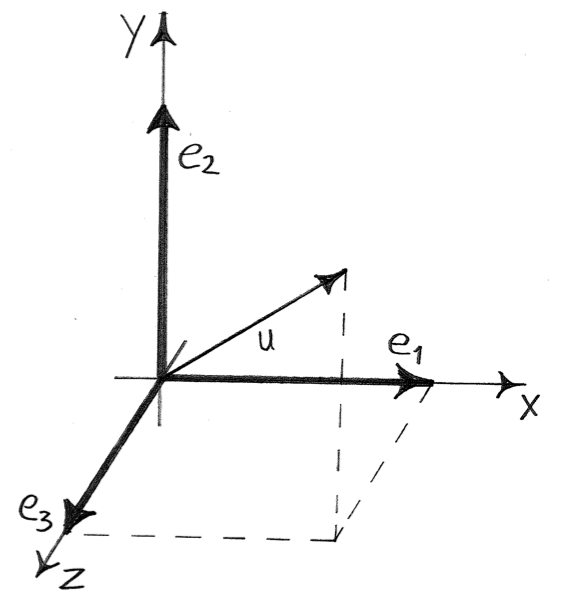
\includegraphics[width=6cm]{./images/mathematics_unprimed_cf.png}
\caption{Vector $u$ in coordinate frame spanned by $e_i$, where $i \ \epsilon \ \lbrace 1,2,3 \rbrace$.}
\label{fig:unprimed_coordinate_frame}
\end{figure}

% Einstein convention
In vector and especially tensor literature a special index
notation if often used. If an index is repeated in a product of
vectors or tensors, summation is implied over the repeated index. This
is also known as the \defit{Einstein Convention} and means the following
is equivalent

\begin{equation}
\delta = a_ib_i \ \ \equiv \ \ \delta = \sum^3_{i=1} a_ib_i \ \
\equiv \ \ \delta = a_1b_1 + a_2b_2 + a_3b_3 
\end{equation} \\

\begin{definition}
\label{def:tensor}
An entity is called a second-order tensor if
it has nine components $T_{ij}$, $i \ \epsilon \ \lbrace 1,2,3
\rbrace$, and $j \ \epsilon \ \lbrace 1,2,3 \rbrace$, in the 
unprimed frame and nine components $T^\prime_{ij}$ in the primed frame and
if these components are related by the characteristic law, defined by:
\begin {equation}
\label{eq:bathe_2_60}
T^\prime_{ij} = P_{il} P_{jm} T_{lm}
\end {equation}
 
\end{definition}

A tensor is defined as an entity,
with components represented in a chosen coordinate frame, that can be
represented in a different coordinate frame, related by the
characteristic law. \\ 

It follows
from definition \vref{def:tensor} that if a tensor equation can be
established in one coordinate frame then it must hold in any other
coordinate frame \citebook{page~502}{book:bathe}. The components of a tensor changes if
the coordinate frame changes. The characteristic law is what 
relates the representation in one coordinate frame to another and it
can also be expressed on matrix form as:

% \begin{equation}
% T^\prime_{mn} e^\prime_m e^\prime_n = T_{kl} e_k e_l
% \end{equation}

% or on matrix from as 

% Def. bathe 2.63 t' = P T P^t
\begin{equation}
\label{eq:primed_stress_tensor}
T^\prime = P \ T \ P^T
\end{equation}

where $P$ is the rotation matrix representing the change of basis from
the primed to the unprimed coordinate frame. The tensor $T$ is  
represented in the unprimed coordinate frame and $P^T$ is the
inverse rotation representing the change of bases from the primed back
to the unprimed coordinate frame. $T^\prime$ is the representation of
the tensor in the primed coordinate frame. \\

Since $P$ is an orthogonal transformation matrix defining a rotation,
the inverse of the transformation equals its transposed matrix
$P^T$ as defined equation \eqref{eq:inverse_equals_transposed}. So the stress tensor
represented in the unprimed coordinate frame can be obtained by:

% Def. bathe 2.64
\begin{equation}
T = P^T \ T^\prime \ P
\end{equation}

According to definition \vref{def:tensor} any tensor can be
represented in a coordinate frame different from the initial
coordinate frame. 

\begin{figure}
  \centering
  \subfloat[Initial unprimed coordinate frame]{
    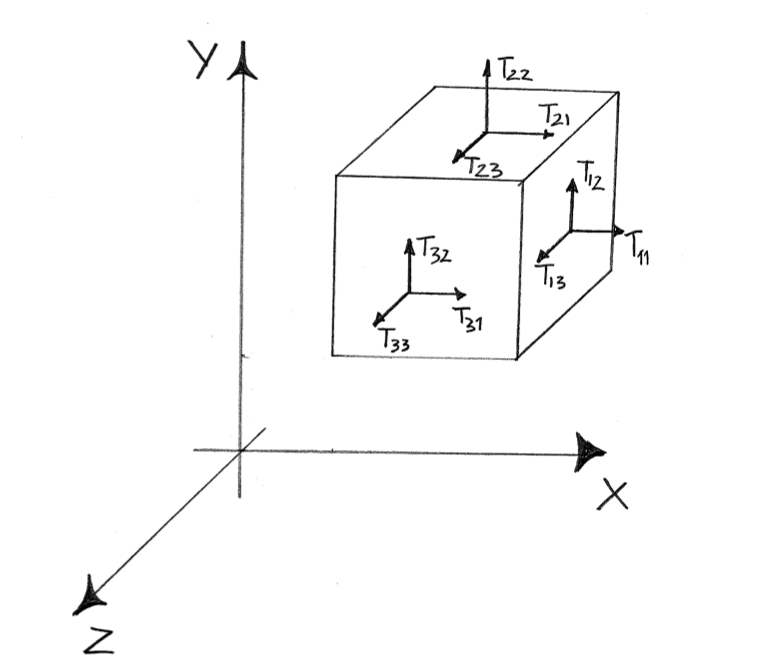
\includegraphics[height=6cm]{./images/mathematics_tensor_transform_a.png}
    \label{fig:mathematics_tensor_transform_a}
  }
  \subfloat[Rotated primed coordinate frame]{
    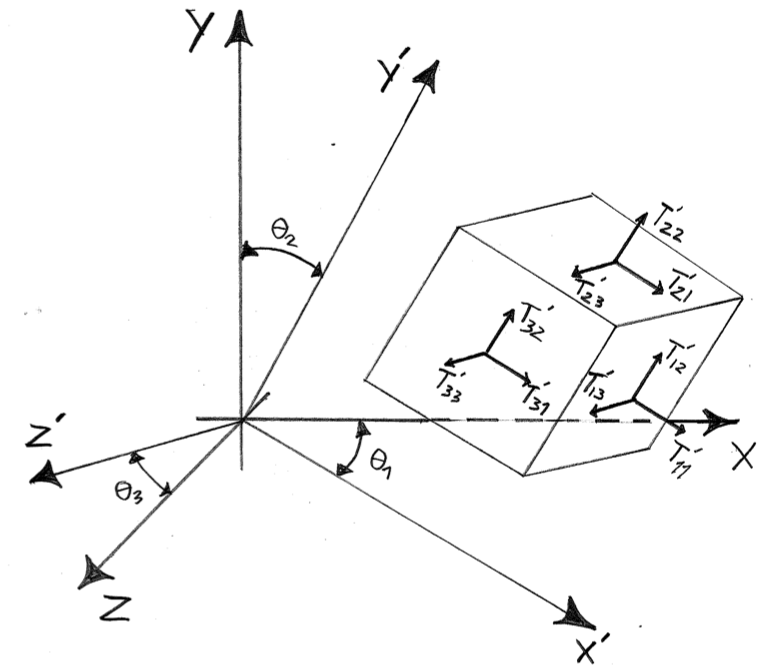
\includegraphics[height=6cm]{./images/mathematics_tensor_transform_b.png}
    \label{fig:mathematics_tensor_transform_b}
  }
  \caption{Transformation of tensor from unprimed to primed coordinate
  frame.}
  \label{fig:tensor_transformation}
\end{figure}


In addition to the unprimed frame, in figure
\vref{fig:mathematics_tensor_transform_a}, consider a primed
coordinate frame. The primed 
coordinate frame spans the same vector space as the unprimed but with
different basis vectors $e^\prime_j$ where $j \ \epsilon \ \lbrace 1,2,3 \rbrace$ as shown in
figure \vref{fig:mathematics_tensor_transform_b}. Now consider any
tensor $T$ represented in the unprimed coordinate frame. The tensor
$T$ can be represented in the primed coordinate frame as
illustrated in figure
\vref{fig:mathematics_tensor_transform_b} through the
relation defined in equation \eqref{eq:primed_stress_tensor},
on matrix form this expands to:

\begin{equation}
  \left[{\begin{matrix} 
        T'_{11} & T'_{12} & T'_{13} \\ 
        T'_{21} & T'_{22} & T'_{23} \\ 
        T'_{31} & T'_{32} & T'_{33} \\ 
      \end{matrix}}\right]
  =
  \left[{\begin{matrix}
        P_{11} & P_{12} & P_{13} \\ 
        P_{21} & P_{22} & P_{23} \\
        P_{31} & P_{32} & P_{33} \\ 
      \end{matrix}}\right]
  \left[{\begin{matrix} 
        T_{11} & T_{12} & T_{13} \\ 
        T_{21} & T_{22} & T_{23} \\ 
        T_{31} & T_{32} & T_{33} \\ 
      \end{matrix}}\right]
  \left[{\begin{matrix} 
        P_{11} & P_{21} & P_{31} \\ 
        P_{12} & P_{22} & P_{32} \\ 
        P_{13} & P_{23} & P_{33} \\ 
      \end{matrix}}\right]
\end{equation}

The diagonal elements of $T'$ represents the scale along the axis of
the primed coordinate frame and the off-diagonal elements represents
shearing.

% In order to discuss this relation in more depth we will
% establish two different coordinate frames and a concrete tensor entity
% to be represented in both.\\

% To establish a second coordinate frame consider, in addition to the unprimed frame in figure
% \vref{fig:unprimed_coordinate_frame}, a primed coordinate frame. The primed
% coordinate frame spans the same vector space as the unprimed but with
% different basis vectors $e^\prime_j$ where $j \ \epsilon \ \lbrace 1,2,3 \rbrace$ as shown in
% figure \vref{fig:unprimed_primed_coordinate_frame}

% % Figure showing primed and unprimed coordinate system
% \begin{figure}
%   \centering
%   \includegraphics[width=6cm]{./images/mathematics_unprimed_primed_cf.png}
% \caption{Different coordinate frames}
% \label{fig:unprimed_primed_coordinate_frame}
% \end{figure}



\subsection{Strain Tensors}
\label{sec:strain_tensors}
As already explained in section \vref{sec:physics_strain} strain
represents the amount of stretch or compression by the relative
distance between two particles in the material body. Strain is a
dimensionless quantity which can be decomposed into normal and
shearing strain. Normal and shearing strain can be represented by a
second order tensor.
Normal strain is the axial stretch or compression represented down the
diagonal as if it was a scaling matrix. Shearing strain is represented
in the off-diagonal components. Altogether we need six components to
represent the entire strain measure, three normal strains and three shearing
strains. As defined in equation \eqref{eq:individual-normal-strain} on
page \pageref{eq:individual-normal-strain} normal strains are obtained by:

\begin{equation*}
\varepsilon_x = \frac{\partial u_x}{\partial x} \hspace{10 mm}
\varepsilon_y = \frac{\partial u_y}{\partial y} \hspace{10 mm}
\varepsilon_z = \frac{\partial u_z}{\partial z}
\end{equation*}

and the three shearing strain, one for each angle between two planes
are defined in equation \eqref{eq:individual-shear-strain}:

\begin{equation*}
  \gamma_{xy} = \frac{\partial u_x}{\partial y} +
  \frac{\partial u_y}{\partial x} \hspace{10 mm}
  \gamma_{xz} = \frac{\partial u_x}{\partial z} +
  \frac{\partial u_z}{\partial x} \hspace{10 mm}
  \gamma_{yz} = \frac{\partial u_y}{\partial z} +
  \frac{\partial u_z}{\partial y}
\end{equation*}

Normal and shearing strain can be represented as a second order tensor:

\begin{equation} 
  E_E =
    \left[\begin{matrix} 
        \varepsilon_x & \gamma_{xy} & \gamma_{xz} \\ 
        \gamma_{yx} & \varepsilon_y & \gamma_{yz} \\ 
        \gamma_{zx} & \gamma_{zy} & \varepsilon_z \\ 
      \end{matrix}\right]
\end{equation}

%  suitable for small deformations. In the infinitesimal strain
% theory small deformations are when the displacement gradients are
% small compared to unity, i.e. $\| \mathbf u\| \ll 1$ and
% $\|\nabla \mathbf u\| \ll 1$. One such strain tensor is the Cauchy's
% strain tensor $E$, obtained by:
 
% \begin{equation}
%   E = \frac{1}{2}\left(\mathbf u\nabla^T + \mathbf
%     u\nabla\right) 
% \end{equation}

% where $u\nabla$ and $u\nabla^T$ is the displacement gradients and its
% transpose, respectively.

% %It is a second order tensor with nine components (only
% %six independent) defined by:

% Using matrix notation it becomes\cite[page~26]{book:mechanical-props-solid-fluid}:

% \begin{equation} 
%   \varepsilon_{ij} =
%     \left[\begin{matrix} 
%         \varepsilon_x & \gamma_{xy} & \gamma_{xz} \\ 
%         \gamma_{yx} & \varepsilon_y & \gamma_{yz} \\ 
%         \gamma_{zx} & \gamma_{zy} & \varepsilon_z \\ 
%       \end{matrix}\right]
%     = 
%     \left[\begin{matrix}
%         \frac{\partial u_x}{\partial x} & 
%         \frac{1}{2} \left(\frac{\partial u_x}{\partial
%             y}+\frac{\partial u_y}{\partial x}\right) & 
%         \frac{1}{2} \left(\frac{\partial u_x}{\partial
%             z}+\frac{\partial u_z}{\partial x}\right) \\ 
        
%         \frac{1}{2} \left(\frac{\partial u_y}{\partial
%             x}+\frac{\partial u_x}{\partial y}\right) & 
%         \frac{\partial u_y}{\partial y} & 
%         \frac{1}{2} \left(\frac{\partial u_y}{\partial
%             z}+\frac{\partial u_z}{\partial y}\right) \\

%         \frac{1}{2} \left(\frac{\partial u_z}{\partial
%             x}+\frac{\partial u_x}{\partial z}\right) &
%         \frac{1}{2} \left(\frac{\partial u_z}{\partial
%             y}+\frac{\partial u_y}{\partial z}\right) &
%         \frac{\partial u_z}{\partial z} \\ 
%       \end{matrix}\right]  
% \end{equation}



\subsection{Stress Tensors}
In continuum mechanics tensors are very useful for representing
e.g. stress. As already explained in section \vref{sec:physics_stress}
stress can be decomposed into normal ($\sigma$) and 
shearing stress ($\tau$). In three dimensions the stress at any point
in the continuum can be completely defined by the stress tensor:

\begin{equation}
\label{eq:stress_tensor}
  S_E = 
  \left[{\begin{matrix} 
        \sigma_x & \tau_{xy} & \tau_{xz} \\ 
        \tau_{yx} & \sigma_y & \tau_{yz} \\ 
        \tau_{zx} & \tau_{zy} & \sigma_z 
      \end{matrix}}\right]
\end{equation}

where the three $\sigma$ components defines the normal stress and the
six $\tau$ defines the shearing stress. Recall from section
\vref{sec:physics_stress} that
since $\tau_{xy} = \tau_{yx}$, $\tau_{yz} = \tau_{zy}$, and $\tau_{zx} =
\tau_{xz}$ the tensor becomes symmetric.


\subsection{Principal Values and Directions}
\label{sec:principal_values_and_directions}
%If for example a strain tensor represents normal and shearing strain
It is often of our interest to determine the directions of the resulting 
strains also known as the \defit{principal directions}. The sizes of the resulting
strains acting in the principal directions are known as the
\defit{principal values}. 
Consider a
strain tensor $E_E$ defining normal and shearing strain. When the
tensor is represented on matrix form we recognize the normal strain
in the axial directions down the diagonal just like a scaling matrix. The shearing is
represented as the off-diagonal components introducing rotation
capabilities into the matrix. Together the normal and shearing strain
forms a transformation matrix mapping vectors from an unprimed to a
primed coordinate frame. The base vectors spanning the primed vector space is
exactly the principle directions we are interested in. Rotating the
unprimed coordinate frame until its base vectors aligns with the base vectors of the
primed coordinate frame, will effectively eliminate the rotation. 
The result from applying normal and shearing strain can hereby be
represented combined as normal strain in the directions of the primed
coordinate frame as illustrated in figure \vref{fig:principal_direction}.

\begin{figure}
  \centering
  \subfloat[Unprimed coordinate frame with shearing strain.]{
    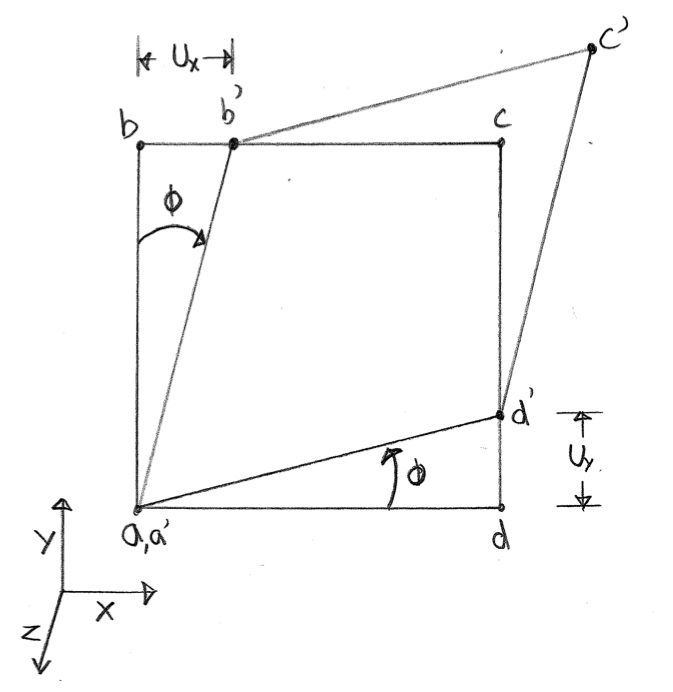
\includegraphics[width=7cm]{./images/mathematics_deformation_shearing_strain_b.png}
    %\label{fig:shearing-strain-one-direction}
  }
  \subfloat[Primed coordinate frame with normal strain.]{
    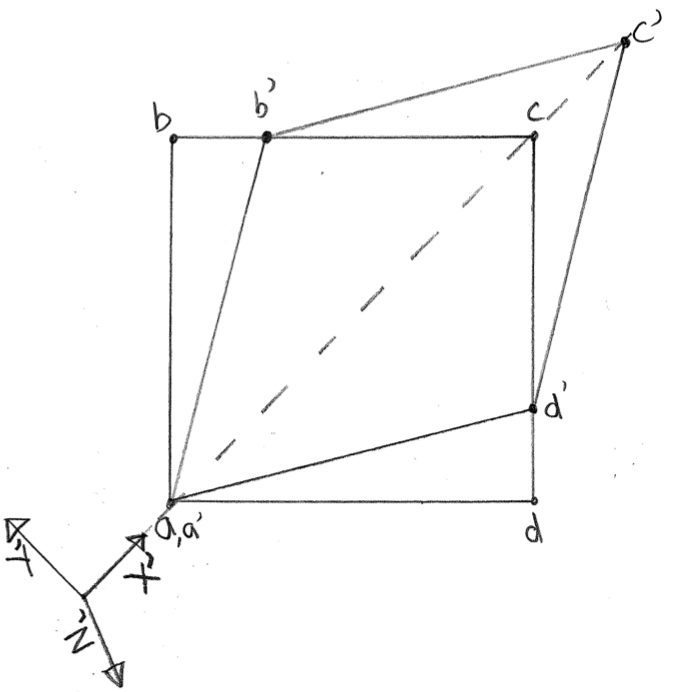
\includegraphics[width=7cm]{./images/mathematics_deformation_shearing_strain_c.png}
    %\label{fig:shearing-strain-two-directions}
  }
  \caption{Shearing strain represented as normal strain.}
  \label{fig:principal_direction}
\end{figure}


The base vectors of the primed coordinate frame
defines the principal directions. The principal values defines the
magnitude of the normal strains that act in the principal directions. 
The solution to the problem of finding the principal directions and values
is equivalent to the solution of the \defit{eigenproblem} as explained
in section \vref{sec:matrix_eigenproblem}. 
%
The eigenvectors of any symmetric tensor
$T$ is by definition three mutually perpendicular vectors. The
eigenvectors defines the
principal directions and the corresponding 
eigenvalues defines the principal values \citebook{page~838}{book:bathe}. 
The three eigenvectors are often referred to as the minimum, medium
and maximum principal directions according to the size of their
corresponding eigenvalues. \\
% The greatest eigenvalue of any tensor $T$ is
% known as the \defit{maximum principle value} and its 
% corresponding eigenvector is know as the \defit{maximum principal
%   direction}. \\


% We will elaborate on the most important property of a tensor, namely the
% fact that any tensor represented in one coordinate frame is related to
% its representation in a different coordinate frame by the
% characteristic law. To clarify on this property the following example
% is simplified to two dimensions but the theory 
% generalizes to $n$ dimensions. Consider stress acting on a square
% represented as a stress tensor in two-dimensional space. 
% In figure \vref{fig:stress_tensor_unprimed_cf} the stress
% tensor is represented in the unprimed coordinate frame. As seen i the
% figure the normal stress components $\sigma_x$ and $\sigma_y$ acts
% in the axial directions here being one in the direction of $x_1$ and
% $y_1$. As explained in section \vref{sec:physics_stress} the stress
% tensor is symmetric which means shearing stress in the $xy$- and
% $yx$-plane are equal ($\tau_{xy}$ = $\tau_{yx}$).
% Shearing stress different from zero causes the square to stretch
% into a parallelogram as illustrated in figure \vref{fig:unit_square_shearing}.

% % Figure showing a square with stress acting on it.
% \begin{figure}
%   \centering
%   \includegraphics[width=12cm]{./images/mathematics_stress_tensor_unprimed_cf.png}
% \caption{Representation of the stress tensor in the unprimed
%   coordinate frame}
% \label{fig:stress_tensor_unprimed_cf}
% \end{figure}
% \{tic}{Redraw figure \vref{fig:stress_tensor_unprimed_cf} using $\sigma$ and $\tau$ notation}

% The tensor $\sigma$ represents stress in
% the unprimed frame. The matrix form is obtained by inserting the normal
% stress $\sigma$ into the matrix diagonal and the shearing stress $\tau$ into the
% off-diagonal entries. Observe how the normal stress components down the diagonal
% forms a matrix similar to the affine scaling matrix defined in section
% \vrefsec{sec:linear_transformation}. By inserting the stress
% components into a stress tensor we obtain

% \begin{equation}
% \sigma \ = \ 
% \begin{bmatrix} 
% \sigma_x & \tau_{xy} \\
% \tau_{yx} & \sigma_y \\
% \end{bmatrix} 
% =
% \begin{bmatrix} 
% 1  & -1 \\
% -1 & 1 \\
% \end{bmatrix} 
% \end{equation} \\

% % The stress tensor $T$ as defined (bathe) represents the change of basis in how
% % the entity is represented

% Consider the stress tensor $\sigma$ represented in the unprimed frame as
% illustrated in figure \vref{fig:stress_tensor_unprimed_cf}. The same
% tensor $\sigma$ can be represented in the primed coordinate, as stated
% in equation \vref{eq:primed_stress_tensor} the relation between to two
% coordinate frames are 

% \begin{displaymath}
% \sigma^\prime = P \ \sigma \ P^T
% \end{displaymath}

% Here $P$ could be expressed as

% % P rotation matrix
% \begin{equation}
% \label{eq:rotation_matrix_p}
% P =
% \begin{bmatrix}
% \cos \theta & \sin \theta \\
% -\sin \theta & \cos \theta \\
% \end{bmatrix}
% \end{equation}

% \vspace{4mm}

% % Example in change of basis
% Assume we want to represent the stress tensor $\sigma$ in the primed
% coordinate frame rotated $45$ degrees counter-clockwise with respect to
% the unprimed frame. The rotation matrix $P$ is used as defined in
% \vref{eq:rotation_matrix_p} with $\theta \ = \ 45$. Since $cos \ 45 \ =
% \ sin \ 45 \ = \ \frac{1}{\sqrt{2}}$, we can rewrite $P$ as

% \begin{equation}
% P =
% \begin{bmatrix}
%  \cos \theta & \sin \theta \\
% -\sin \theta & \cos \theta \\
% \end{bmatrix}
% =
% \frac{1}{\sqrt{2}} 
% \begin{bmatrix}
%  1 & 1 \\
% -1 & 1 \\
% \end{bmatrix}
% \end{equation}

% \vspace{4mm}
% Due to the fact that both matrix $P$ and $P^T$ brings
% $\frac{1}{\sqrt{2}}$ to equation \vref{eq:primed_stress_tensor} and
% since $(\frac{1}{\sqrt{2}})^2 = \frac{1}{2}$ we obtain

% \begin{equation}
% \sigma^\prime = \frac{1}{2}
% \begin{bmatrix}
% 1 & 1 \\
% -1 & 1 \\
% \end{bmatrix}
% \begin{bmatrix}
% 1 & -1 \\
% -1 & 1 \\
% \end{bmatrix}
% \begin{bmatrix}
% 1 & -1 \\
% 1 & 1 \\
% \end{bmatrix}
% =
% \begin{bmatrix}
% 0 & 0 \\
% 0 & 2 \\
% \end{bmatrix}
% \end{equation} 

% \vspace{4mm}
% Notice how the shearing stress, represented in the off-diagonal
% elements of tensor $\sigma^\prime$, are all zeros. The normal stresses
% represented in the diagonal are $0$ and $2$. The stress tensor $\sigma^\prime$ 
% represents the same stress but in the primed coordinate frame. The
% primed coordinate axes are now aligned with the {\it principal
%   directions} of the stress. The diagonal values of $\sigma^\prime$ are 
% known as the {\it principal values} and define the normal stress
% acting in the principal directions. \\

% Rotating the coordinate frame by
% $45^\circ$ did by coincidence make the primed coordinate axis align with the
% principal directions of the stress. 


% Assume we are interested in
% determining the principal directions and values of an arbitrary
% tensor. The solution to this problem is equivalent to the solution of
% the {\it eigenproblem} as explained in section
% \vref{sec:matrix_eigenproblem}.\\

% A second order tensor in
% three-dimensions, like \vref{eq:stress_tensor} on page \pageref{eq:stress_tensor}, is a
% symmetric $3 \times 3$ matrix with three 
% eigenvalues. The eigenvalues are the principle stresses and
% their corresponding eigenvectors are the directions of the principal
% stress\cite{book:bathe}.


\section{The Matrix Eigenproblem}
\label{sec:matrix_eigenproblem}
Solving the matrix eigenproblem means finding eigenvalues and
their corresponding eigenvectors for a given matrix. Finding the
eigenvalues and eigenvectors reduces to the solution of linear
equations \citeabook{book:leon} as defined below \\

\begin{definition}
\label{def:eigenproblem}
Let $\mathbf{A}$ be an $n \times n$ matrix. A scalar $\lambda$ is said
  to be an \textbf{eigenvalue} or a \textbf{characteristic value} of
  $\mathbf{A}$ if there exists a nonzero vector $\mathbf{v}$ such that
  $\mathbf{A} \mathbf{v} = \lambda \mathbf{v}$. The vector
  $\mathbf{v}$ is said to be an \textbf{eigenvector} or a
    \textbf{characteristic vector} belonging to $\lambda$.
\end{definition}


The equation $A v = \lambda v$ can also be written as
\begin{equation}
\label{eq:def_eigenproblem_equal_zero}
(A - \lambda I) v =  0
\end{equation}
According to definition \vref{def:eigenproblem} $\lambda$ is an eigenvalue of $A$
if and only if the corresponding vector $v$ is nonzero. Equation
\eqref{eq:def_eigenproblem_equal_zero} has a nonzero 
solution of $v$ if and only if $det(A - \lambda I) = 0$ is
satisfied, this equation is
also known as the \defit{characteristic equation} for matrix $A$. \\

Expanding the
determinant leaves us with an polynomial of $n$-degree for the
$\lambda$ term. This polynomial is also known as the
\defit{characteristic polynomial}. The characteristic polynomial will have
exactly $n$ roots being the eigenvalues from which we can find $n$
independent eigenvectors. \\

% reference to why we never has to deal with complex numbers
\textbf{Example} \\
Consider a matrix $A$ defined to be:
\begin{equation*}
A = 
\begin{bmatrix} 
  1 & 1 \\ 
  -2 & 4 
\end{bmatrix} 
\end{equation*}

Finding the eigenvalues and eigenvectors means solving equation
\eqref{eq:def_eigenproblem_equal_zero}. By insertion we obtain:

\begin{equation*}
( A - \lambda I) v =
\begin{bmatrix} 
  1 & 1 \\ 
  -2 & 4 
\end{bmatrix} 
\begin{bmatrix} 
x_1 \\ x_2 
\end{bmatrix} 
-
\begin{bmatrix} 
\lambda & 0 \\
0 & \lambda  
\end{bmatrix} 
\begin{bmatrix} 
x_1 \\ x_2 
\end{bmatrix}
= 
\begin{bmatrix} 
0 \\ 0 
\end{bmatrix}  
\end{equation*}

which is equivalent to:

\begin{align}
\label{eq:eigenvalue_one}
(1 - \lambda) x_1 + x_2 & = 0 \\
\label{eq:eigenvalue_two}
(4 - \lambda) x_2 - 2x_1 & = 0
\end{align}

With only two equations and three unknowns a third condition is
needed. As previously stated $\lambda$ is an eigenvalue of matrix 
$A$ if and only if vector $v$ has a nonzero solution. If matrix $A$ is
singular the equation \eqref{eq:def_eigenproblem_equal_zero} will have a
nontrivial solution. From the characteristic polynomial we obtain a
third condition:

\begin{equation} 
det(A - \lambda I) = det
\begin{pmatrix} 
  1 - \lambda & 1 \\ 
  -2 & 4 - \lambda 
\end{pmatrix}
= 0
\end{equation}

which expands to:
\begin{equation}
(1 - \lambda)(4 - \lambda) + 2 = 6 - 5 \lambda + \lambda^2 = (\lambda
- 3)(\lambda - 2) = 0
\end{equation}

Obvious $\lambda = 2$ and $\lambda = 3$ is a valid solution here.
Standard techniques for finding roots in a given
polynomial exists. Having established the two eigenvalues we still need to find their
corresponding and independent eigenvectors satisfying the equation $A
v = \lambda v$. By inserting $\lambda = 2$ into equation
\eqref{eq:eigenvalue_one} and \eqref{eq:eigenvalue_two} we obtain:

\begin{align}
% multiply-defined \label{eq:eigenvalue_one_reduced}
-x_1 + x_2 & = 0 \\
% multiply-defined \label{eq:eigenvalue_two_reduces}
-2x_1 + 2x_2 & = 0
\end{align}

By looking at the coefficients and signs of the vector components $x_1$
and $x_2$ we see that the equation is satisfied with the base solution:

\begin{equation}
\begin{bmatrix}
x_1 \\ x_2
\end{bmatrix}
=
\begin{bmatrix}
1 \\ 1
\end{bmatrix}
\end{equation}

Any non-zero multiple of $[1,1]^T$ is an eigenvector belonging to
$\lambda = 2$. Eigenvector $[1,1]^T$ is said to be a basis for the
\defit{eigenspace} corresponding to $\lambda = 2$.
A scalar $\lambda$ with corresponding vector $v$ satisfying 
$A v = \lambda v$ defines an \defit{eigenpair}. \\ 

The second independent eigenvector corresponding to $\lambda = 3$ is
found just like before through insertion of $\lambda = 3$ into equation
\eqref{eq:eigenvalue_one} and \eqref{eq:eigenvalue_two} hereby obtaining:

\begin{align}
\label{eq:eigenvalue_one_reduced}
-2x_1 + x_2 & = 0 \\
\label{eq:eigenvalue_two_reduces}
-2x_1 + x_2 & = 0
\end{align}

in order to satisfy the equation the solution must be:

\begin{equation}
\begin{bmatrix}
x_1 \\ x_2
\end{bmatrix}
=
\begin{bmatrix}
1 \\ 2
\end{bmatrix}
\end{equation}

We have now solved the eigenproblem for matrix $A$ by finding the two
eigenvalues and their corresponding eigenvectors. The solution written as
eigenpairs:

\begin{equation}
(2, \begin{pmatrix} 1 \\ 1 \end{pmatrix} ),
( 3, \begin{pmatrix} 1 \\ 2 \end{pmatrix} )
\end{equation}

Due to the fact that any second order tensor can be represented on
matrix form, the eigenproblem can be solved for second order tensors
by a similar approach to the one just shown. More general techniques
for solving the eigenproblem exists but will not be further discussed
here. \\

%All tensors of our interest are symmetric by definition. In section
%\todo{ref. to stress tensors defining symmetry} we shall elaborate why
%this is the case. 

%Tensor visualization is further elaborated in section ??.

%Since any multiple of each eigenvector is a valid solution to the
%eigenproblem we can not distinguish what is front and back on each
%plane. So from three plane normals we can span eight vector spaces,
%one for each quadrant in a three-dimensional coordinate
%frame. There exists many techniques for tensor visualization,
%generally it is 